\chapter{Dataset and Task Setup}
\justify
The CLEF JOKER Task 1 dataset contains a humor-focused English corpus and query-relevance annotations.

\section{Dataset Summary}
\begin{table}[H]
\centering
\begin{tabular}{|l|c|}
\hline
Corpus size & 77,658 documents \\\hline
Training queries & 12 \\\hline
Training qrels & 660 \\\hline
Test queries & 219 \\\hline
Primary metric & MAP@1000 \\\hline
\end{tabular}
\caption{Dataset statistics used in this project.}
\end{table}

\section{Task Characteristics}
\begin{itemize}
    \item Queries are very short and ambiguous.
    \item Relevance is humor-sensitive and context-dependent.
    \item Candidate generation requires balancing recall and precision.
\end{itemize}

\section{Dataset Visualization (LaTeX Figure)}
\begin{figure}[H]
\centering
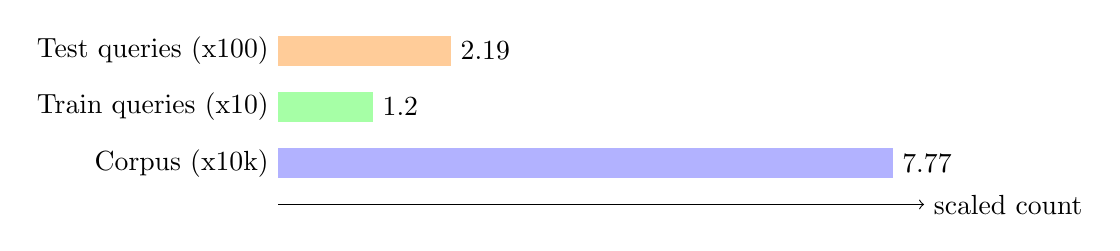
\begin{tikzpicture}[x=1cm,y=0.55cm]
\fill[blue!30] (0,0) rectangle (7.8,0.7);
\fill[green!35] (0,1.3) rectangle (1.2,2.0);
\fill[orange!40] (0,2.6) rectangle (2.19,3.3);
\node[left] at (0,0.35) {Corpus (x10k)};
\node[left] at (0,1.65) {Train queries (x10)};
\node[left] at (0,2.95) {Test queries (x100)};
\node[right] at (7.8,0.35) {7.77};
\node[right] at (1.2,1.65) {1.2};
\node[right] at (2.19,2.95) {2.19};
\draw[->] (0,-0.6) -- (8.2,-0.6) node[right]{scaled count};
\end{tikzpicture}
\caption{Scaled bar-style visualization of dataset composition.}
\end{figure}
